\section{Il Problema dell'Object Detection}

\subsection{Computer Vision}
La Computer Vision è una branca dell'intelligenza artificiale che si occupa dello sviluppo di metodi che consentano ai computer di interpretare e comprendere il mondo visivo in modo simile agli esseri umani. Questa capacità è cruciale per sviluppare applicazioni avanzate che richiedono l'analisi e l'elaborazione delle immagini e dei video. La Computer Vision comprende quindi le basi teoriche, gli algoritmi e i modelli matematici necessari per acquisire, elaborare, analizzare e comprendere le immagini digitali, con l'obiettivo di estrarre informazioni significative dall'ambiente visivo.

Tra i problemi centrali di cui si occupa la Computer Vision, troviamo:
\begin{itemize}
  \item \textbf{Image Recognition}: Identificare e classificare oggetti o scene all'interno di un'immagine. Questo include compiti come il riconoscimento facciale, il riconoscimento di oggetti e il riconoscimento di azioni.
  \item \textbf{Object Detection}: Localizzare e identificare oggetti di interesse all'interno di un'immagine, determinando la loro posizione attraverso bounding box. Questo è fondamentale per applicazioni come il tracciamento degli oggetti, la guida autonoma e la sorveglianza.
  \item \textbf{Semantic Segmentation}: Dividere un'immagine in segmenti che corrispondono a oggetti o regioni con caratteristiche simili. Questo aiuta a comprendere la struttura dell'immagine a livello di pixel.
  \item \textbf{Scene Recognition}: Interpretare e descrivere l'intera scena rappresentata in un'immagine, inclusi gli oggetti presenti e le loro relazioni spaziali.
  \item \textbf{Pose Estimation}: Determinare la posizione e l'orientamento di un oggetto nello spazio tridimensionale a partire da immagini bidimensionali.
  \item \textbf{3D Reconstruction}: Ricostruire modelli tridimensionali di oggetti o scene a partire da immagini bidimensionali. Questo è cruciale per applicazioni come la realtà aumentata e la robotica.
  \item \textbf{Object Tracking}: Seguire il movimento di uno o più oggetti attraverso una sequenza di immagini o video. Questo è essenziale per applicazioni come la sorveglianza video e la guida autonoma.
  \item \textbf{Super-Resolution}: Migliorare la risoluzione di un'immagine partendo da versioni a bassa risoluzione, utile per migliorare la qualità visiva e per analisi più dettagliate.
\end{itemize}

Questi problemi sono alla base di molte applicazioni pratiche della Computer Vision e sono spesso interconnessi.


\subsection{Object Detection}
L'Object Detection è quindi uno dei problemi fondamentali della Computer Vision. Esso riguarda la localizzazione e identificazione di uno o più oggetti di interesse all'interno di un'immagine o di un video. A differenza dell'Image Recognition, che si limita a classificare un'intera immagine, l'Object Detection deve determinare sia la presenza degli oggetti sia le loro posizioni precise.

\begin{figure}[ht]
    \centering
    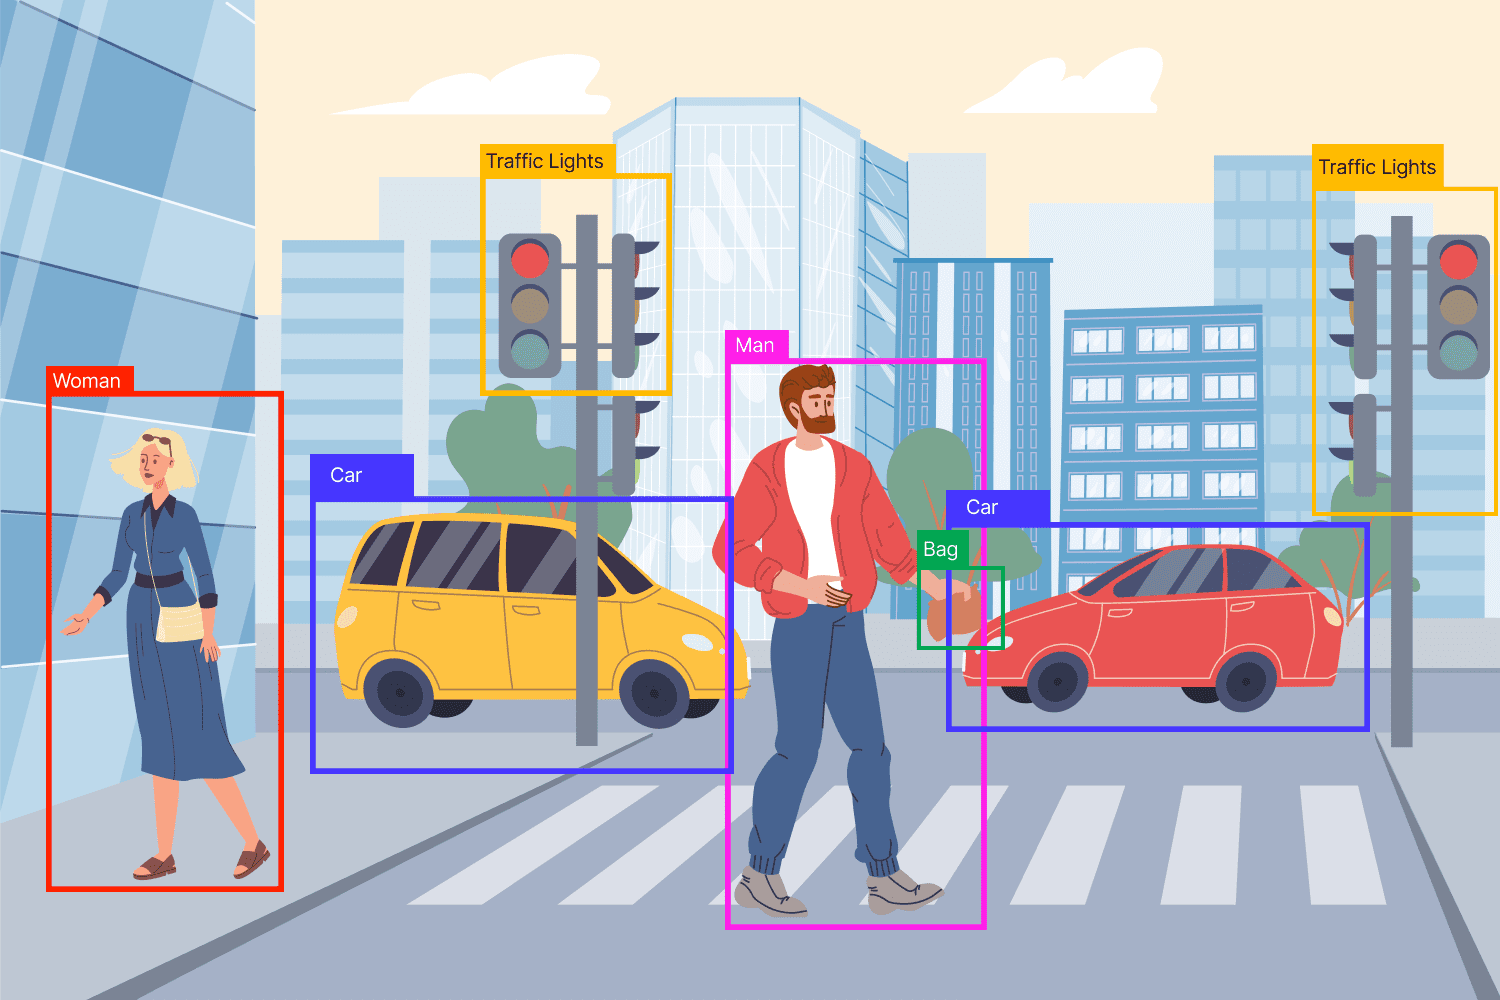
\includegraphics[width=0.75\textwidth]{files/capitoli/1-object-detection/assets/object-detection-example.png}
    \caption{\label{fig:object-detection-example}Esempio di Object Detection di un'immagine\cite{1}}
\end{figure}

L'Object Detection ha due obiettivi principali:
\begin{itemize}
  \item \textbf{Localizzazione}: Determinare la posizione degli oggetti all'interno dell'immagine, solitamente rappresentata da bounding box (rettangoli che contornano gli oggetti).
  \item \textbf{Classificazione}: Identificare la classe a cui appartiene ogni oggetto rilevato (ad esempio persona, automobile, animale, ecc...).
\end{itemize}

Questi obiettivi richiedono algoritmi capaci di elaborare immagini complesse e di generare previsioni accurate e efficienti in termini di calcolo.

L'Object Detection è pertanto un processo complesso che combina diverse fasi, ognuna delle quali gioca un ruolo cruciale nel garantire l'accuratezza e l'efficienza del sistema complessivo.

I principali passaggi coinvolti nell'Object Detection sono:
\begin{itemize}
  \item \textbf{Feature Extraction}
  \item \textbf{Bounding Box Prediction}
  \item \textbf{Classification}
  \item \textbf{Non-Maximum Suppression (NMS)}
\end{itemize}

\subsubsection{Feature Extraction}
La fase di Feature Extraction è cruciale nell'Object Detection, in quanto le caratteristiche estratte rappresentano la base su cui si fondano le successive fasi di localizzazione e classificazione. Questa fase coinvolge l'uso di reti neurali convoluzionali (CNN) per identificare caratteristiche rilevanti delle immagini, come bordi, texture, forme e colori.

\begin{figure}[ht]
    \centering
    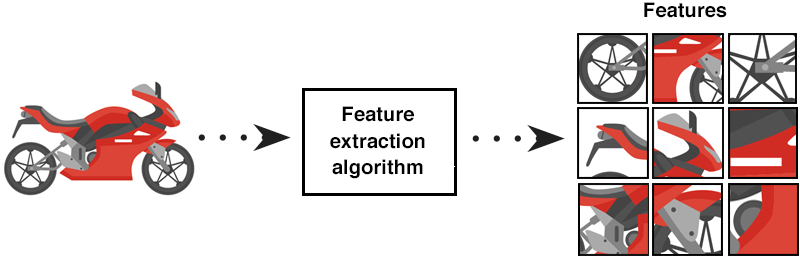
\includegraphics[width=1\textwidth]{files/capitoli/1-object-detection/assets/feature-extraction.png}
    \caption{\label{fig:feature-extraction}Esempio di Feature Extraction di un'immagine\cite{2}}
\end{figure}

\newpage

Le CNN sono una classe di reti neurali composte da vari layer di diversi tipi, ciascuno con una funzione specifica:
\begin{itemize}
  \item \textbf{Convolutional Layers}: estraggono caratteristiche locali come bordi, angoli e texture tramite l'applicazione di filtri (kernel) sull'immagine di input. Ogni kernel convoluziona l'immagine generando una feature map che evidenzia la presenza di specifici pattern.
  \item \textbf{Activation Layers}: applicano una funzione di attivazione non lineare (ad esempio, ReLU - Rectified Linear Unit) dopo ogni convolutional layer, la quale introduce non-linearità nel modello, permettendo alla rete di apprendere rappresentazioni più complesse.
  \item \textbf{Pooling Layers}: riducono le dimensioni spaziali delle feature map (tipicamente mediante operazioni di max pooling o average pooling), riducendo così il numero di parametri e computazioni nella rete, e introducendo invarianza rispetto alle traslazioni. Questo aiuta a rendere il modello più robusto e a prevenire l'overfitting.
\end{itemize}

\begin{figure}[ht]
    \centering
    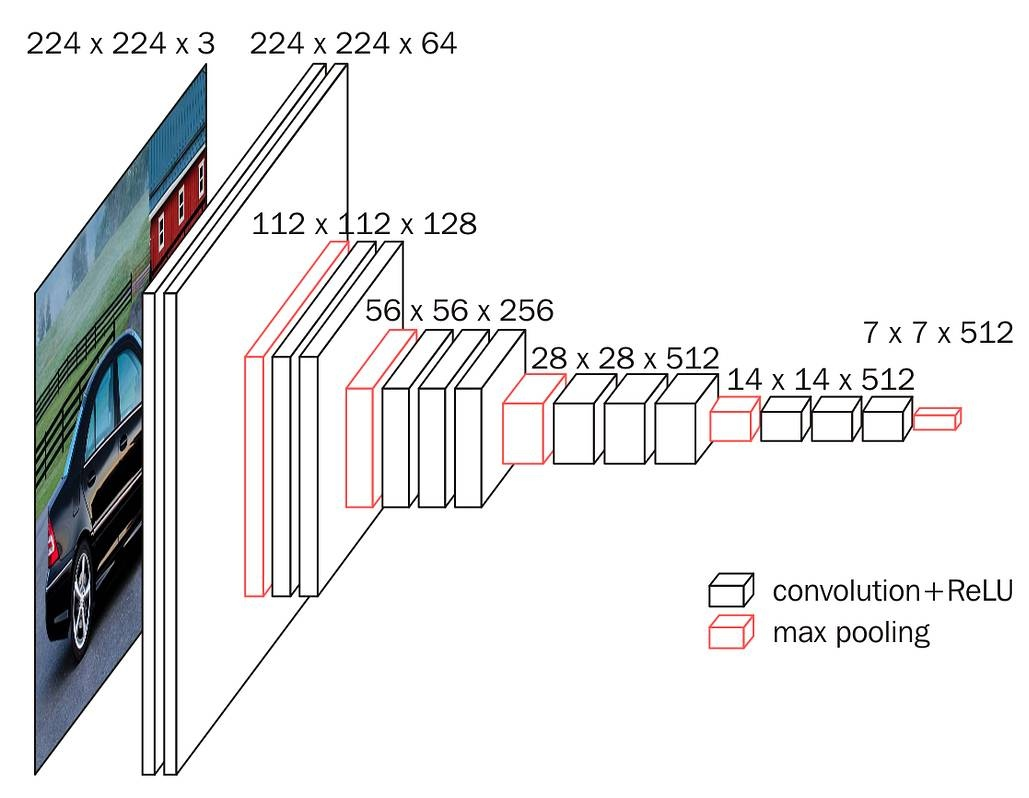
\includegraphics[width=0.6\textwidth]{files/capitoli/1-object-detection/assets/feature-extraction-layers.jpg}
    \caption{\label{fig:feature-extraction-layers}Layers della CNN adibiti alla Feauture Extraction\cite{3}}
\end{figure}

Quando un'immagine viene data in input ad una CNN, questa passa attraverso la serie di convolutional e pooling layers. I primi convolutional layers tendono a rilevare caratteristiche di basso livello, come bordi e texture, mentre i successivi catturano caratteristiche di livello più alto, come parti di oggetti e forme complete. L'uso di multipli convolutional layers permette quindi alla rete di costruire una rappresentazione gerarchica delle caratteristiche dell'immagine.

Il risultato finale della fase di Feature Extraction è una serie di feature maps che catturano informazioni spaziali e di contesto sull'immagine. Queste feature maps sono poi utilizzate nei passaggi successivi per la predizione delle bounding box e la classificazione degli oggetti.

\subsubsection{Bounding Box Prediction e Classification}
La predizione delle bounding box e la classificazione degli oggetti sono due passaggi cruciali nell'Object Detection. A seconda dell'architettura del modello, questi passaggi possono essere eseguiti separatamente o simultaneamente.

Nei modelli basati su region proposals, come R-CNN e le sue varianti, la predizione delle bounding box e la classificazione avvengono in due passaggi distinti:

\begin{enumerate}
  \item \textbf{Generazione delle Proposal Regions}: in questa fase, il modello utilizza algoritmi come il Selective Search o una Region Proposal Network (RPN) per generare un insieme di region proposals, che sono regioni dell'immagine candidate a contenere oggetti. Il Selective Search utilizza tecniche di segmentazione per trovare regioni simili, mentre l'RPN è una rete neurale che produce direttamente proposte di regioni.

\begin{figure}[ht]
    \centering
    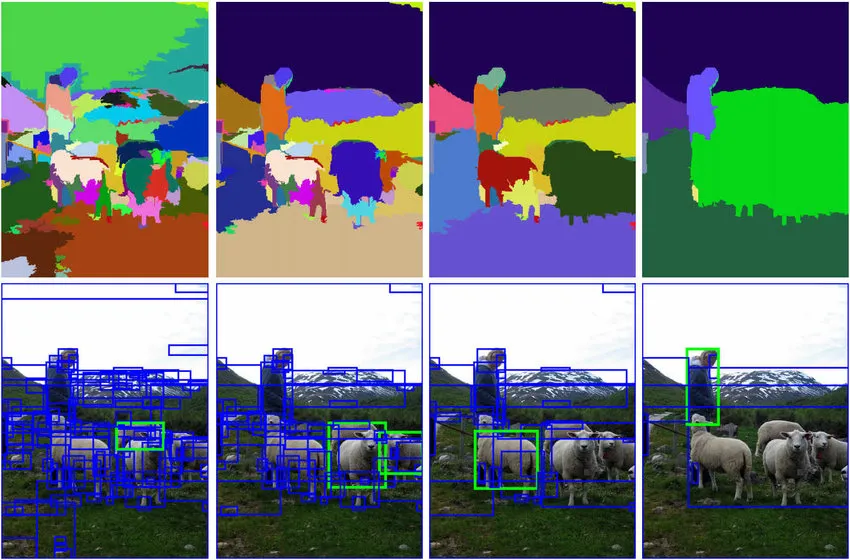
\includegraphics[width=0.8\textwidth]{files/capitoli/1-object-detection/assets/selective-search-region-proposals.png}
    \caption{\label{fig:selective-search-region-proposals}Esempio di generazione delle Proposal Regions con l'algoritmo Selective Search\cite{4}}
\end{figure}
  
  \item \textbf{Predizione delle Bounding Box e Classificazione}: ogni region proposal viene estratta dalle feature maps e passata attraverso una CNN che effettua la predizione delle bounding box precise e la classificazione degli oggetti. In R-CNN, questo passaggio viene eseguito separatamente per ciascuna region proposal, mentre in varianti come Fast R-CNN e Faster R-CNN, queste operazioni vengono ottimizzate per migliorare la velocità e l'efficienza.
\end{enumerate}

Nei modelli single-shot, come SSD e YOLO, la predizione delle bounding box e la classificazione degli oggetti avvengono simultaneamente in un unico passaggio.

Questo approccio è caratterizzato dai seguenti passaggi chiave:
\begin{enumerate}
  \item \textbf{Suddivisione in Griglia}: dopo la feature extraction, l'immagine di input viene suddivisa in una griglia di dimensioni predefinite, ad esempio 7x7 o 13x13, a seconda delle specifiche del modello.
  \item \textbf{Predizione delle Bounding Box}: per ogni cella della griglia, il modello utilizza le feature maps per predirre un insieme di bounding box, ciascuna definita da:
  \begin{itemize}
    \item Coordinate (x, y) del centro della bounding box rispetto alla cella della griglia
    \item Altezza e larghezza (h, w) della bounding box, normalizzate rispetto alle dimensioni dell'immagine
    \item Un punteggio di confidenza (objectness score) che riflette la probabilità che la bounding box contenga un oggetto e la precisione con cui la bounding box delimita l'oggetto
  \end{itemize}
  \item \textbf{Classificazione}: oltre alle coordinate e all'objectness score, per ogni bounding box viene predetta una distribuzione di probabilità sulle classi degli oggetti. Il modello quindi stima la probabilità che l'oggetto contenuto nella bounding box appartenga a ciascuna delle classi target.
  \item \textbf{Calcolo del Punteggio Finale}: l'objectness score per ogni bounding box viene moltiplicato per le probabilità di classe per ottenere un punteggio finale per ogni combinazione di bounding box e classe. Questo punteggio finale aiuta a determinare quali bounding box e classi saranno considerate nella fase finale di rilevamento.
\end{enumerate}

\begin{figure}[ht]
    \centering
    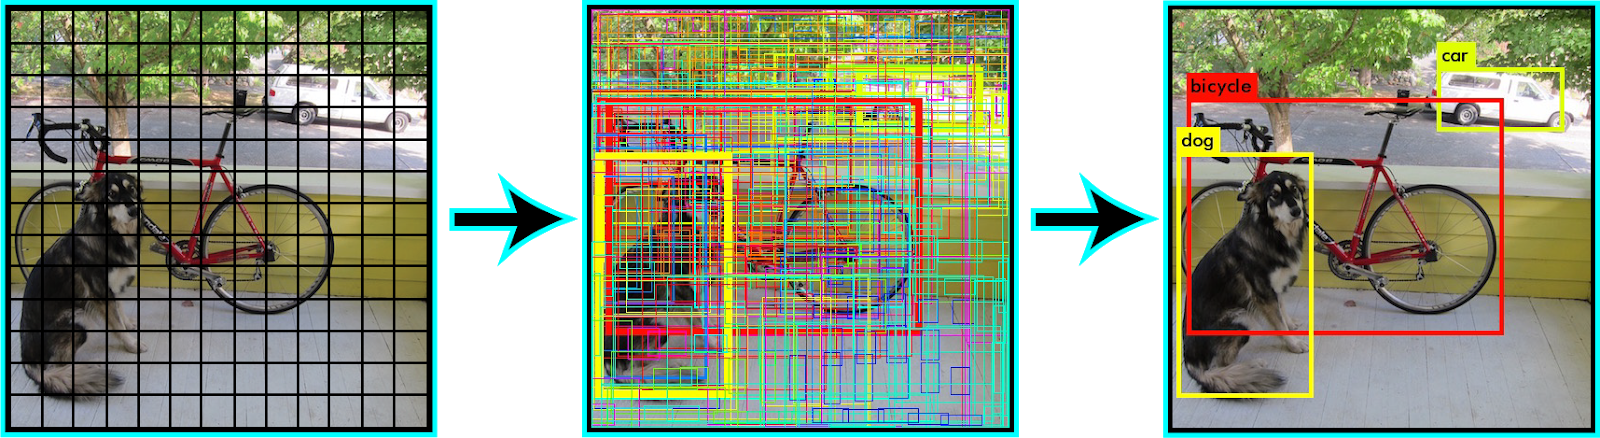
\includegraphics[width=0.8\textwidth]{files/capitoli/1-object-detection/assets/single-shot-grid.png}
    \caption{\label{fig:single-shot-grid}Bounding Box Prediction e Classification dei modelli single-shot\cite{5}}
\end{figure}


\newpage

\subsubsection{Non-Maximum Suppression}
La Non-Maximum Suppression (NMS) è una tecnica essenziale utilizzata nei modelli di Object Detection per ridurre le proposte ridondanti di bounding box o regioni che coprono gli oggetti rilevati. 
Questa viene applicata dopo la fase di generazione delle proposte (bounding box o regioni), le quali vengono valutate e ordinate in base a un punteggio di confidenza, che rappresenta la probabilità che una proposta contenga un oggetto.

L'NMS identifica e rimuove le proposte che hanno un'elevata sovrapposizione con altre proposte di punteggio più alto, mantenendo solo quelle più accurate e significative.

\begin{figure}[ht]
    \centering
    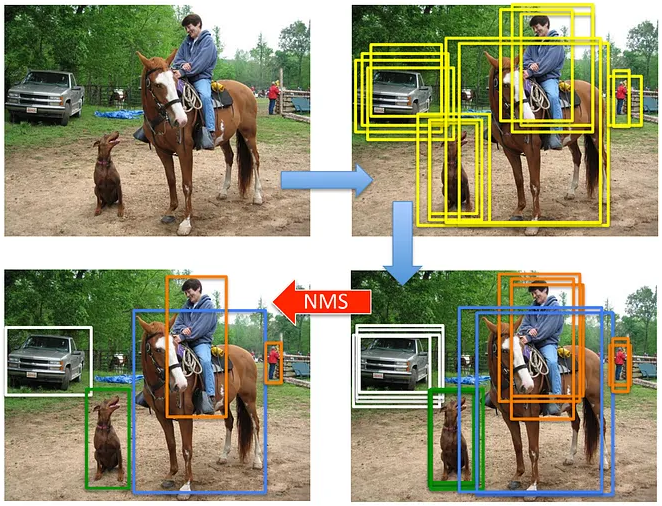
\includegraphics[width=0.7\textwidth]{files/capitoli/1-object-detection/assets/nms-example.png}
    \caption{\label{fig:nms-example}Esempio di rimozione delle bounding box ridondanti tramite Non-Maximum Suppression\cite{5}}
\end{figure}

\newpage
